\documentclass[12pt,a4paper]{article}
\usepackage[utf8]{inputenc}
\usepackage{graphicx}
\graphicspath{{../Images/}}
\usepackage{amsmath}
\usepackage{amsfonts}
\usepackage{amssymb}
\usepackage{hyperref}
\usepackage[margin=1in]{geometry}
\usepackage{subfig}
\usepackage{float}
\usepackage{xcolor}
\usepackage{listings}
\definecolor{dkgreen}{rgb}{0,0.6,0}
\definecolor{gray}{rgb}{0.5,0.5,0.5}
\definecolor{mauve}{rgb}{0.58,0,0.82}

\lstset{frame=tb,
  backgroundcolor=\color[rgb]{0.93,0.93,0.93},
  language=Python,
  aboveskip=3mm,
  belowskip=3mm,
  showstringspaces=false,
  columns=flexible,
  basicstyle={\small\ttfamily},
  numbers=none,
  numberstyle=\tiny\color{gray},
  keywordstyle=\color{blue},
  commentstyle=\color{dkgreen},
  stringstyle=\color{mauve},
  breaklines=true,
  breakatwhitespace=true,
  tabsize=3
}

\author{Thibaut Marmey}

\title{Notes de cours CADL - session-2}

\begin{document}
	\maketitle

\begin{scriptsize} \begin{itemize}
\item The basic components of a neural network
\item How to use gradient descent to optimize parameters of a neural network
\item How to create a neural network for performing regression
\end{itemize}\end{scriptsize}

\begin{normalsize}
\tableofcontents
\end{normalsize}

\section{Introduction}
\subsection{Generalities}
\begin{itemize}
\item Use data and gradient descent to teach the network what the values of the parameters of the network should be.
\item Idea of machine learning : letting the machine learn from the data.
\item We are interested in letting the computer figure out what representations it needs in order to better describe the data and some objective we've defined.
\end{itemize}
\subsection{Gradient Descent}
\begin{itemize}
\item Operations of the network are meant to transform the input data into something meaningful that we want the network to learn about.
\item Parameters of the NW are random so output is random as well.
\item If we need specific output, we can use "Gradient Descent" : way to optimize set of parameters.
\end{itemize}
\subsection{Defining Cost}
\begin{itemize}
\item Mesure of the "error"
\item Exemple : recognize apple or orange. Random network spit ou random 0s or 1s for apples and oranges. We can define :
\begin{itemize}
\item if the network predicts a 0 for an orange, then the error is 0. If the network predicts a 1 for an orange, then the error is 1. 
\item And vice-versa for apples. If it spits out a 1 for an apple, then the error is 0. If it spits out a 0 for an apple, then the error is 1. 
\end{itemize}
\item Defining error in terms of our parameters :
\begin{equation} error = network(image) - true\_label 
\end{equation}
\begin{equation} network(image) = predicted\_label
\end{equation}
\begin{equation} E = f(X) - y
\end{equation}
\end{itemize}
\subsection{Minimizing Error}
\begin{itemize}
\item Feed the network many images (100 for e.g) to see what the network is doing on average.
\item Changing network's parameters can have effect on the error.
\item The error provides a "training signal" or a measure of the "loss" or our network.
\item Assumptions in assuming our funtion is continuous and differentiable. 
\item Gradiant descent in a nutshell : "Error", "Cost", "Loss", or "Training Signal"
\end{itemize}
\subsection{Backpropagation}
\begin{itemize}
\item  The gradient is just saying, how does the error changes at the current set of parameters.
\item To figure out what is the gradian we use backpropagation. Whatever differences that output has with the output we wanted it to have, gets \textit{backpropagated} to every single param in our network.
\item Backprop is an effective way to find the gradient. Uses the \textit{chain rule} to find the gradian of the error.
\item \textit{y = mx + b} linear function. The slope or gradian is \textit{m}.
\item The process described : 
\begin{equation} \theta = \theta - \eta * \nabla_\theta * J(\theta)
\end{equation}
\begin{itemize}
\item $\theta$ : parameters
\item $\nabla$ : gradient, with repect to parameters $\theta$, $\nabla_\theta$
\item J : error
\item $\eta$ : learning rate describes how far along this gradient we should travel, typically value between 0.01 to 0.00001
\end{itemize}
\end{itemize}
\subsection{Local Minima/Optima and learning Rate}
\begin{itemize}
\item Dilemma : find a local or global minima.
\item The NW may have million of parameters, so the problem becomes more and more difficult.
\item Wize choice of the learning rate : 
\begin{itemize}
\item To small we dont get any better cost where we started
\item To big the cost goes up and down
\end{itemize} 
\end{itemize}

\section{Creating a Neural Network}
\subsection{Exemple with sine wave}
\begin{itemize}
\item Input X output y
\item Here the input is values in an interval instead of images like before.
\item The exemple is to create sine wave with uniform noise and create a neural network that is able to discover the sine wave.
\begin{lstlisting}
# Create data : sine wave with random noise in the interval
n_obs = 1000
xs = np.linscape(-n, n, n_obs)
ys = np.sin(xs) + np.random.uniform(-0.5,0.5,n_obs)
plt.scatter(xs, ys)
\end{lstlisting}
\item Train the NW to give any value on the x axis and have the value it should be on the y axis. (fundamental idea of regression : predicting some continuous output value given some continuous input value)
\end{itemize}
\subsection{Defining cost}
\begin{itemize}
\item Use of placeholder to define input and output values. Those variables will filled at the computation of the graph.
\begin{lstlisting}
X = tf.placeholder(tf.float32, name='X')
Y = tf.placeholder(tf.float32, name='Y')
\end{lstlisting}
\item Create session and define the parameters center and close to 0 with \\
\textit{tf.random\_normal(nb\_values, stddev=).eval()}
\begin{lstlisting}
sess = tf.InteractiveSession()
n = tf.random_normal([1000], stddev=0.1).eval()
\end{lstlisting}
\item Create \textbf{variables} using \textit{tf.Variable}, it does need an initial value or we can call an initializer.
\item Define two \textit{tf.Variable} for weight and bias
\begin{lstlisting}
W = tf.Variable(tf.random_normal([1], dtype=tf.float32, stddev=0.1), name='weight')
B = tf.Variable(tf.constant([0], dtype=tf.float32), name='bias')
# Scale input placholder X
Y_pred = X * W + B
\end{lstlisting}
\item Use gradient descent to learn what the best value of \textit{W} and \textit{b}.
\item Before that we have to know how to measure what the \textit{best} mean for what we try to do.
\item Let's define the absolute \textit{distance(val1, val2)} from the predicted value to the assumed sine wave value.
\begin{lstlisting}
cost = distance(Y_pred, tf.sin(X))
\end{lstlisting}
\item We calculate the mean of the cost we have for every observation
\begin{lstlisting}
cost = tf.reduce_mean(distance(Y_pred, tf.sin(X))
\end{lstlisting}
\end{itemize}
\subsection{Training Parameters}
\begin{itemize}
\item Use tensorflow optimizer 
\begin{lstlisting}
optimizer = tf.train.GradientDescentOptimizer(learning_rate=0.01).minimize(cost)
\end{lstlisting}
\item Run the optimizer
\begin{lstlisting}
with tf.Session() as sess:
   #initilization of all the tf.Variable
   sess.run(tf.global_varables_initializer())
   prev_training_cost = 0.0
   for it_i in range(n_iterations):
      sess.run(optimizer, feed_dict={X:xs, Y:ys})
      training_cost = sess.run(cost, feed_dict={X:xs}) #...,session=sess)
      
      # each 10 iterations
      if it_i % 10 == 0:
         ys_pred = Y_pred.eval(feed_dict={X:xs})
         # print stuff like training_cost and plots
      
      if np.abs(prev_training_cost - training_cost < 0.000001):
         break # if local minima found
        
      prev_trianing_cost = training_cost
\end{lstlisting}
\item The output doesn't look like a sine wave at all. Actually it's only a line.
\item Training vs Testing : Have to learn more about the different between training and testing networks.
\end{itemize}
\subsection{Stochastic and Mini Batch Gradient Descent}
\begin{itemize}
\item Tricks to find the best local minima : using \textit{mini-batches} of size \textit{batch\_size}.
\begin{lstlisting}
idxs = np.arrange(100) # it will be changed to make it random
batch_size = 10
n_batches = idxs // batch_size
\end{lstlisting}
\item Look some random subset of the datase because neural networks love order and would use it to its advantage. But order is irrelevant to our problem.
\begin{lstlisting}
idxs = np.random.permutation(idxs)
\end{lstlisting}
\item Generalise the entire dataset. We modify the code which runs the optomizer to include the mini-batches program.
\begin{lstlisting}
idxs = np.random.permutation(range(len(xs)))
n_batches = len(idxs) // batch_size
for batch_i in range(n_batches):
   idxs_i = idxs[batch_i * batch_size: (batch_i+1) * batch_size]
   sess.run(optimizer, feed_dict={X:xs[idxs_i], Y:ys[idxs_i]})
training_cost = sess.run(cost, feed_dict={X:xs, Y:ys})
\end{lstlisting}
We get a better result : the line has a curve but it doesn't look like a sine wave.
\item This method is :
\begin{itemize}
\item Mini-batches : small pieces of data where we perform gradient descent
\item Stochastic : the order of the data is dandomized
\end{itemize}
\item Use a function of training
\begin{lstlisting}
def train(X, Y, Y_pred, n_iterations=100, batch_size=200, learning_rate=0.02):
\end{lstlisting}
\item To get better result we can have a bigger set of parameters.
\item We are going to multiply our input by 100 values, creating an "inner layer" of 100 neurons.
\begin{itemize}
\item Define \textit{tf.Variables} : Weights (multiplication) and biais (addition)
\begin{lstlisting}
n_neurons = 100
W = tf.Variable(tf.random_normal([1,n_neurons], stddev=0.1))
b = tf.Variable(tf.constant(0), dtype=tf.float32, shape=[n_neurons])
\end{lstlisting}
\item Operation with matrix and add every neuron's output
\begin{lstlisting}
h = tf.matmul(tf.expand_dims(X, 1), W) + b)
Y_pred = tf.reduce_sum(h, 1)
\end{lstlisting}
\item Retrain with new Y\_pred
\begin{lstlisting}
train(X, Y, Y_pred)
\end{lstlisting}
\end{itemize}
\item It takes longer to compute and the result is not better. Our function is still linear but the cost is going up and down : good sign = we can reduce the learning rate
\item Input's Representation : important to consider the kind of input we are working on. We don't treat the types of data in the same way like :
\begin{itemize}
\item sound using discrete fourier transform
\item text using word histograms
\end{itemize}
\end{itemize}
\subsection{Over vs. Underfitting}
\begin{itemize}
\item To approximate curve function we use polynomial function. We will try to learn the influence of each degree of this function
\begin{lstlisting}
Y_pred = tf.Variable(tf.random_normal([1]), name='bias')
for pow_i in range(1,4):
   W = tf.Variable(
       tf.random_normal([1], stddev=0.1), name='weight_%d' % pow_i)
   Y_pred = tf.add(tf.multiply(tf.pow(X, pow_i), W), Y_pred)
\end{lstlisting}
\end{itemize}
\subsection{Introducing Nonlinearities / Activation Function}
\begin{itemize}
\item Use of non-linear functions also called activation functions. In every complex DL algorithm there are series of linear, followed by nonlinear operations.
\item There are 3 functions used the most : \textit{tanh(), sigmoid(), relu()}\\
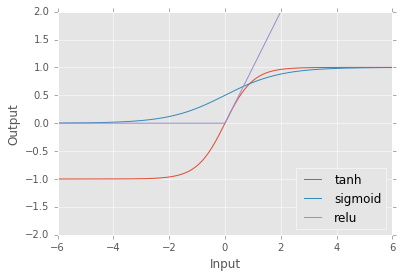
\includegraphics[scale=0.5]{nonLinearities}
\item We modify the matrix multiplication by adding the non-linearity
\begin{lstlisting}
h = tf.nn.tanh(tf.multiply(tf.expland_dims(X,1), W) + b, name='h')
\end{lstlisting}
\item \textbf{Fully-connected network} : every neuron is multiplied by every single input value. We multiply our input by a matrix, add a bias, and then apply a non-linearity.
\end{itemize}
\subsection{Going Deeper}
\begin{itemize}
\item Give useful name within \textit{scopes}. Otherwise the names of the operations are not helpful.
\begin{lstlisting}
W = tf.get_variable( name='W', shape=[n_input, n_output],
    initializer=tf.random_normal_initializer(mean=0.0, stddev=0.1))
\end{lstlisting}
\item This new initializer will create new random value when\\
\textit{sess.run(tf.global\_variables\_initializer())} is called
\item Possible to visualize the network using \textbf{Tensorboard}.
\end{itemize}

\section{Image Inpainting}
\subsection{Description}
\begin{itemize}
\item This NW will try to demonstrate how the NW we've created bedfore can realize more complicated tasks on the following image :\\
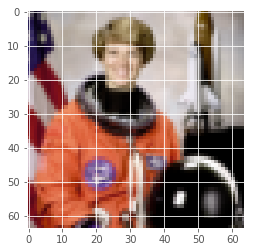
\includegraphics[scale=0.3]{inPainting}
\item We will teach the NW to go from the location on an image frame to a particular color.
\item Given any position in an image, the NW will need to learn what color to paint.
\item Start
\begin{itemize}
\item Declare input and output
\begin{lstlisting}
# positions in the image
xs = []
# coresponding colors
ys = []
\end{lstlisting}
\item Storage
\begin{lstlisting}
# for loop on the image
xs.append([row_i, col_i])
ys.append(img[row_i,col_i])
xs = np.array(xs)
ys = np.array(ys)
\end{lstlisting}
\item Normalization
\begin{lstlisting}
xs = (xs - np.mean(xs)) / np.std(xs)
\end{lstlisting}
\end{itemize}
\item Goint to use regression to predict the value of a pixel biven its (row, col) position.
\item Place input and output in placeholder in which we specify the partially their shape
\begin{lstlisting}
X = tf.placeholder(tf.float32, shape=[None,2], name='X')
Y = tf.placeholder(tf.float32, shape=[None,3], name='Y')
\end{lstlisting}
\end{itemize}
\subsection{Building the Network}
\begin{itemize}
\item We are going to create a multi-layers NW.
\item We take the \textit{linear()} function created previously.
\begin{lstlisting}
def linear(X, n_input, n_output, activation=None, scope=None):
    with tf.variable_scope(scope or "linear"):
        W = tf.get_variable(
            name='W',
            shape=[n_input, n_output],
            initializer=tf.random_normal_initializer(mean=0.0, stddev=0.1))
        b = tf.get_variable(
            name='b',
            shape=[n_output],
            initializer=tf.constant_initializer())
        h = tf.matmul(X, W) + b
        if activation is not None:
            h = activation(h)
        return h
\end{lstlisting}
\item We use for loop to create the NW
\begin{lstlisting}
n_neurons = [2, 64, 64, 64, 64, 64, 64, 3]
current_input =X
for layer_i in range(1, len(n_neurons)):
   current_input = linear(
      X = current_input, # returned value of the function
      n_input = n_neurons[layer_i - 1],
      n_output = n_neurons[layer_i],
      activation = tf.nn.relu if (layer_i+1) < len(n_neurons) else None,
      scope = 'layer_'+str(layer_i))
Y_pred = current_input
\end{lstlisting}
\end{itemize}
\subsection{Training}
\begin{itemize}
\item Define the cost
\begin{lstlisting}
cost = tf.reduce_mean(tf.reduce_sum(distance(Y_pred, Y), 1))
\end{lstlisting}
\item Use another opitmizer \textit{AdamOptimizer} (in general better than \textit{GradientDescentOptimizer}). 
\begin{lstlisting}
optimizer = tf.train.AdamOpitmizer(0.001).minimize(cost)
\end{lstlisting}
\item Ready to launch the process
\begin{itemize}
\item Start the session
\begin{lstlisting}
with tf.Session() as sess:
\end{lstlisting}
\item Initialize variables (W and  b) in the graph so we can use them
\begin{lstlisting}
sess.run(tf.global_variables_initializer())
prev_training_cost = 0.0
\end{lstlisting}
\item Loop for over number of iterations :
\begin{lstlisting}
for it_i in range(n_iterations):
\end{lstlisting}
\begin{itemize}
\item Permutation of the input (randomness used for the optimizer)
\begin{lstlisting}
idxs = np.random.permutation(range(len(xs)))
\end{lstlisting}
\item Computation of the number of mini-batches
\begin{lstlisting}
n_batches = len(idxs) // batch_size
\end{lstlisting}
\item Loop for over the number of mini-batches
\begin{lstlisting}
for batch_i in range(n_batches):
\end{lstlisting}
\begin{itemize}
\item Take the subinterval of input of the current mini-batch
\begin{lstlisting}
idxs_i = idxs[batch_i*batch_size: (batch_i+1)*batch_size]
\end{lstlisting}
\item Run the optimizer by feeding input X and output Y to calculate the parameters W and b
\begin{lstlisting}
sess.run(optimizer, feed_dict={X:xs, Y:ys})
\end{lstlisting}
\end{itemize}
\item Compute the cost to visualize the progression
\begin{lstlisting}
training_cost = sess.run(cost, feed_dict={X:xs, Y:ys})
print(it_i, training_cost)
\end{lstlisting}
\end{itemize}
\item Visualize the result by plotting
\begin{lstlisting}
ys_pred = Y_pred.eval(feed_dict={X:xs}, session=sess)
img = np.clip(ys_pred.reshape(img.shape), 0, 255).astype(np.uint8)
\end{lstlisting}
\end{itemize}
\item The entire code
\begin{lstlisting}
n_iterations = 500
batch_size = 50
with tf.Session() as sess:
    # Here we tell tensorflow that we want to initialize all
    # the variables in the graph so we can use them
    # This will set W and b to their initial random normal value.
    sess.run(tf.global_variables_initializer())

    # We now run a loop over epochs
    prev_training_cost = 0.0
    for it_i in range(n_iterations):
        idxs = np.random.permutation(range(len(xs)))
        n_batches = len(idxs) // batch_size
        for batch_i in range(n_batches):
            idxs_i = idxs[batch_i * batch_size: (batch_i + 1) * batch_size]
            sess.run(optimizer, feed_dict={X: xs, Y: ys})

        training_cost = sess.run(cost, feed_dict={X: xs, Y: ys})
        print(it_i, training_cost)

        if (it_i + 1) % 20 == 0:
            ys_pred = Y_pred.eval(feed_dict={X: xs}, session=sess)
            fig, ax = plt.subplots(1, 1)
            img = np.clip(ys_pred.reshape(img.shape), 0, 255).astype(np.uint8)
            plt.imshow(img)
            plt.show()
\end{lstlisting}
\end{itemize}

\section{Homework}
\subsection{Goals}
\begin{itemize}
\item Learn how to create Neural Network
\item Learn to use a NN to paint a image
\item Apply creative thinking to the inputs, outputs and definition of a NW
\end{itemize}
\subsection{Part One : Fully Connected Network}
\begin{itemize}
\item Create the operations for connecting an input to a NW, defined by a \textit{tf.placeholder}, to a series of fully connected, or linear, layers using the formula :
\begin{equation}
\textbf{H} = \phi(\textbf{XW + b})
\end{equation}
\begin{itemize}
\item \textbf{H} : output layer representing the "hidden" activations of a network
\item $\phi$ : linearity
\item \textbf{X} : input to that layer
\item \textbf{W} : layer's weight matirx
\item \textbf{b} : layer's bias
\end{itemize}
\item The part \textbf{XW} is the most compicated part of the equation scaling and rotating our input.
\item By stacking a lot of "linear" + "nonlinear" operations in a series, we can create a \textbf{deep neural network}.
\item Choising nonlinearities : trial and error. Depends on the normalization scheme : the expected output.
\item Keep in mind the functions \textit{relu}, \textit{sigmoïd} and \textit{tanh} for their properties expecially for the final output layer of the NW
\subsubsection{Code}
\begin{itemize}
\item Create a placeholder for the input \textbf{X}
\begin{lstlisting}
X = tf.placeholder(dtype=tf.float32, shape=[None, 2], name='X')
\end{lstlisting}
\item Create the paramaters \textbf{W} and \textbf{b}
\begin{lstlisting}
W = tf.get_variable(dtype=tf.float32, shape=[2,20], intializer=tf.random_normal_initializer, name='W')
b = tf.get_variable(dtype=tf.float32, shape=[20], intializer=tf.constant_initializer, name='b')
\end{lstlisting}
\item Matrix multiplication \textbf{XW} and addition with \textbf{b} : XW + b
\begin{lstlisting}
h = tf.matmul(X, W)
h = tf.nn.bias_add(h,b)
\end{lstlisting}
\item Nonlinearity \textit{relu}
\begin{lstlisting}
h = tf.nn.relu(h, name='relu')
\end{lstlisting}
\item New "linear" function using \textit{tf.get\_scope}. If there is already a variable created with the same name, TF will raise an exception. Consider 3 solutions :
\begin{itemize}
\item In an interactive console
\begin{lstlisting}
tf.reset_default_graphe()
\end{lstlisting}
\item Typo error creating another layer with the same name
\item Should use context manager when creating graphs and running sessions
\begin{lstlisting}
g = tf.Graph()
with tf.Session(graph=g) as sess:
   Y_pred, W = linerar(X, 2, 3, activation=tf.nn.relu)
\end{lstlisting}
\end{itemize}
\end{itemize}
\end{itemize}

\subsection{Part Two : Image Painting Network}
\begin{itemize}
\item Load an image
\begin{lstlisting}
img = plt.imshow(dirname)
\end{lstlisting}
\item Collect location of pixel and the related (R,G,B) colors using for loops. Convert the lists of input and output to arrays \textit{np.array()}
\item Normalize the input \textit{xs}
\begin{lstlisting}
xs = (xs - np.mean(xs)) / np.std(xs)
\end{lstlisting}
\item Create \textit{placeholder} for the input and the true output
\begin{lstlisting}
# first reset the graph
tf.reset_default_graph()
X = tf.placeholder(dtype=tf.float32, shape=[None,2], name='X')
Y = tf.placeholder(dtype=tf.float32, shape=[None,3], name='Y')
\end{lstlisting}
\item Create 8 layers of neurons : \{2, 20, 20, 20, 20, 20, 20, 3\}
\begin{itemize}
\item 2 is the input layer
\begin{equation}
H_1 = \phi(XW_1 + b_1)
\end{equation}
\item All the 20 are the hidden layers
\begin{equation}
H_{i} = \phi(H_{i-1}W_i + b_i)
\end{equation}
\item 3 is the output layer
\begin{equation}
Y_{pred} = \phi(H_6W_7 + b_7)
\end{equation}
\end{itemize}
\subsubsection{Cost function}
\begin{itemize}
\item 
\end{itemize}
\end{itemize}




\end{document}
